%%%%%%%%%%%%%%%%%%%%%%%%%%%%%%%%%%%%%%%%%
% Original author:
% Linux and Unix Users Group at Virginia Tech Wiki
% (https://vtluug.org/wiki/Example_LaTeX_chem_lab_report)
% Modified by: Hector F. Jimenez S, for the Digital Electronics Laboratory.
% License:
% CC BY-NC-SA 3.0 
%%%%%%%%%%%%%%%%%%%%%%%%%%%%%%%%%%%%%%%%%
%----------------------------------------
%	PACKAGES AND DOCUMENT CONFIGURATIONS
%---------------------------------------
\documentclass[paper=a4, fontsize=12pt]{article} 		% A4 paper and 11pt font size
\usepackage[T1]{fontenc} 								% Use 8-bit encoding that has 256 glyphs
%\usepackage{fourier}		 							% Use the Adobe Utopia font for the document 
\usepackage[spanish,english]{babel}						% Spanish Language, templates uses some sections in english.
\selectlanguage{spanish}								% main language.
\PassOptionsToPackage{spanish}{babel}
%\renewcommand{\figurename}{Figura}						% Force rename of figure.
%\renewcommand{\figurename}{Fig.}
\usepackage[figurename=Fig.]{caption}
\usepackage[utf8]{inputenc}								% tildes for spanish language.
\usepackage{amsmath,amsfonts,amsthm} 					% Math packages.
\usepackage{minted}										% For syntax highlighting.
\usepackage{float}										% Image will be in the same place as you want.!!! x-/
\usepackage{sectsty} 									% Allows customizing section commands
\allsectionsfont{\centering \normalfont\scshape}	   	% Make all sections centered, the default font and small caps
\usepackage{hyperref}
\hypersetup{											%Setups the false color and borders.
    colorlinks=false,
    pdfborder={0 0 0},
}
\newcommand\fnurl[2]{%									% set a simple and quick footnote command and include url.
\href{#2}{#1}\footnote{\url{#2}}%	
}
\usepackage{graphicx}									% Import easyly images.
\graphicspath{ {./images/} }							% Where to look for the images.
\DeclareGraphicsExtensions{.pdf,.png,.jpg}				% Graphics Extension to be used
\usepackage[notes,backend=biber]{biblatex-chicago}		% Bibliography and references.
\bibliography{biblio}									% bibliography filename.
\usepackage{fancyhdr} 									% Custom headers and footers
\pagestyle{fancyplain} 									% Makes all pages in the document conform to the custom headers and footers
\fancyhead{} 											% No page header
\fancyfoot[L]{} 										% Empty left footer
\fancyfoot[C]{} 										% Empty center footer
\fancyfoot[R]{\thepage} 								% Page numbering for right footer
\renewcommand{\headrulewidth}{0pt} 						% Remove header underlines
\renewcommand{\footrulewidth}{0pt} 						% Remove footer underlines
\setlength{\headheight}{13.6pt} 					    % Customize the height of the header
\numberwithin{equation}{section}						% Number equations within sections (i.e. 1.1, 1.2, 2.1, 2.2 instead of 1, 2, 3, 4)
%\numberwithin{figure}{section} 						% Number figures within sections (i.e. 1.1, 1.2, 2.1, 2.2 instead of 1, 2)
\numberwithin{table}{section} 							% Number tables within sections (i.e. 1.1, 1.2, 2.1, 2.2 instead of 1, 2, 3, 4)
\setlength\parindent{0pt} 								% Removes all indentation from paragraphs
%\newcommand{\horrule}[1]{\rule{\linewidth}{#1}} 		% Create horizontal rule command with 1 argument of height
%%%%%%%%%%%%%%%%%%%%
%Title Section
%%%%%%%%%%%%%%%%%%%%%
\title{Desarrollo de un Turnero Digital\\ 
Usando FPGA's \\
Laboratorio de Electrónica Digital\\Módulo: 2} 			% Title
%\horrule{0.5pt} \\[0.4cm] 								% Thin top horizontal rule	Title rule
%\huge Assignment Title \\ 								% The assignment title
%\horrule{2pt} \\[0.5cm] 								% Thick bottom horizontal rule
\author{												% Authors begin.
Héctor F. \textsc{Jiménez S.}\\
\texttt{hfjimenez@utp.edu.co} \\
\texttt{PGP KEY ID: 0xB05AD7B8}
\and
Sebastian \textsc{Zapata}\\
\texttt{sebastzapata93@gmail.com }\\
\texttt{PGP KEY ID: 0xfffff}
\and 
Jorge Mario \textsc{Gil}\\
\texttt{jorgemario.gil@utp.edu.co}\\
\texttt{PGP KEY ID: 0xfffff}
} 												       % End of  Author name
\date{}    						                       % Date for the report, this will hide the \today.

\begin{document}
\maketitle                      			           % Insert the title, author and date
\begin{center}
\begin{tabular}{l r}								   % two column to
Fecha de Entrega: & Agosto, 2016 \\				   % Ramiro's Details.
Profesor: & Ing.Msc(c) Ramiro Andres Barrios Valencia
\end{tabular}
\end{center}
%%%%%%%%%%%	
% Let's start the document.
%%%%%%%%%%%	
\section{Objetivos}
\begin{itemize}
  \item Desarrollar la unidad de control para la generación de mensajes a aravés del arreglo de cuatro display de siete segmentos.
  \item Desarrollar modulo para la conversion para pasar a BCD. 
  
\end{itemize}
$\\$
%%%%%%%%%%%	
% Theory Marc! 
%%%%%%%%%%%	
\section{Marco Teórico}
\begin{figure}[H]
  \centering
     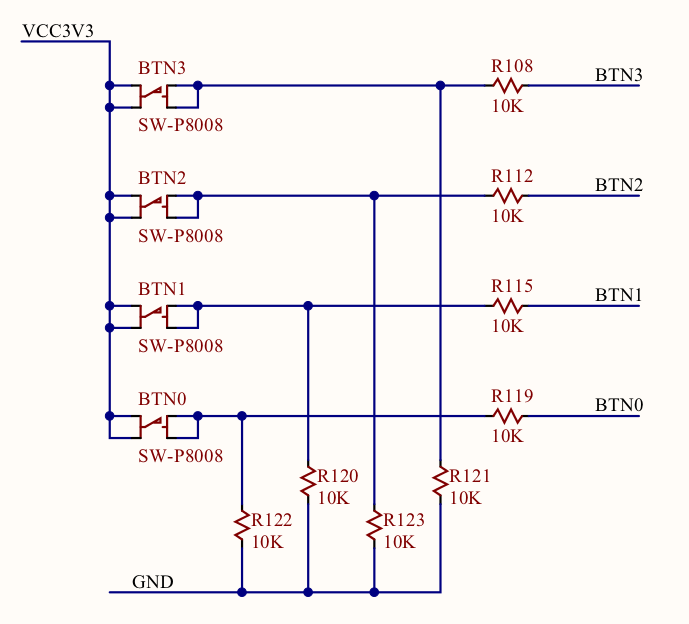
\includegraphics[width=0.5\textwidth]{btn1.png}
  \caption{Esquema provisto en el esquemático, 4 pulsadores.}
    \label{fig:btn}
\end{figure}


\section{Control Modulo de Siete Segmentos}
\section{Código VHDL}
Descripción del Pseudo código para el módulo anti rebote:
\begin{minted}{vhdl}
 1 Setup a counter variable, initialise to zero.
 2 Setup a regular sampling event, perhaps using a timer. Use a period of about 1ms.
\end{minted}
$$\\$$
$$\\$$
$$\\$$
$$\\$$
$$\\$$
$$\\$$
$$\\$$
$$\\$$
%\inputminted{vhdl}{./Code/debounce.vhd}
$$\\$$
$$\\$$
$$\\$$
$$\\$$
$$\\$$
$$\\$$
\section{Prácticas Experimentales}
Se realizaran pruebas sobre la placa nexys2 para verificar que el programa realiza la tarea necesaria.

\section{Anexos}
los demás archivos son adicionales que resuelven la misma implementación, se encuentran en el repositorio \texttt{github.com\/heticor915\/DigitalElectronicsLab\/tree\/master\/Reports\/Module2\/}
\textit{Nota}: Las referencias utilizadas se encuentran en los pies de página. Si requiere de manera detallada estas contacte con \emph{miembros del equipo.}
\end{document}
